\documentclass[9pt]{beamer}
% Created By Gouthaman KG
%~~~~~~~~~~~~~~~~~~~~~~~~~~~~~~~~~~~~~~~~~~~~~~~~~~~~~~~~~~~~~~~~~~~~~~~~~~~~~~
% Use roboto Font (recommended)
\usepackage[sfdefault]{roboto}
\usepackage[utf8]{inputenc}
\usepackage[T1]{fontenc}
%~~~~~~~~~~~~~~~~~~~~~~~~~~~~~~~~~~~~~~~~~~~~~~~~~~~~

\usepackage{upquote}  % straight single quotes
\usepackage{subfig}   % for \subfloat
\usepackage{setspace} % for custom line spacing

%~~~~~~~~~~~~~~~~~~~~~~~~~~~~~~~~~~~~~~~~~~~~~~~~~~~~~~~~~~~~~~~~~~~~~~~~~~~~~~
% Define where theme files are located. ('/styles')
\usepackage{styles/fluxmacros}
\usefolder{styles}
% Use Flux theme v0.1 beta
% Available style: asphalt, blue, red, green, gray 
\usetheme[style=asphalt]{flux}
%~~~~~~~~~~~~~~~~~~~~~~~~~~~~~~~~~~~~~~~~~~~~~~~~~~~~~~~~~~~~~~~~~~~~~~~~~~~~~~

%~~~~~~~~~~~~~~~~~~~~~~~~~~~~~~~~~~~~~~~~~~~~~~~~~~~~~~~~~~~~~~~~~~~~~~~~~~~~~~
% Extra packages for the demo:
\usepackage{booktabs}
\usepackage{colortbl}
\usepackage{ragged2e}
\usepackage{schemabloc}
\usepackage{hyperref}
\usepackage{caption}
\usepackage{fancyvrb}
\DeclareMathOperator*{\argmax}{\arg\!\max}
\DeclareMathOperator*{\argmin}{\arg\!\min}
\usebackgroundtemplate{
\includegraphics[width=\paperwidth,height=\paperheight]{"assets/background"}}%change this to your preferred background for the presentation.
%~~~~~~~~~~~~~~~~~~~~~~~~~~~~~~~~~~~~~~~~~~~~~~~~~~~~~~~~~~~~~~~~~~~~~~~~~~~~~~

%~~~~~~~~~~~~~~~~~~~~~~~~~~~~~~~~~~~~~~~~~~~~~~~~~~~~~~~~~~~~~~~~~~~~~~~~~~~~~~

\graphicspath{{assets/}}
\newcommand{\ve}[1]{\mathbf{#1}}
% Informations
\title{Linear Discriminant Analysis}
\subtitle{MATH 156 Final Project}

\usepackage[style=ieee,backend=biber]{biblatex}
\addbibresource{bib}

\author{Aatmun Baxi, Abhijith Vemulapati, Andy Chen, Johnny Mo}
\institute{University of California, Los Angeles}

\titlegraphic{assets/ucla_logo.png}
% \titlegraphic{assets/gkg.png} %change this to your preferred logo or image(the image is located on the top right corner).
%~~~~~~~~~~~~~~~~~~~~~~~~~~~~~~~~~~~~~~~~~~~~~~~~~~~~~~~~~~~~~~~~~~~~~~~~~~~~~~

\begin{document}

% Generate title page
\titlepage
\section{Overview}
\begin{frame}{Overview}
\setstretch{1.618}
\begin{itemize}
    \item LDA can be used a multiclass classification model or a supervised dimensionality reduction routine
    \item LDA is a dimensionality reduction technique similar to PCA. Unlike PCA, it is supervised and it focuses on class separability. 
    \item Assumes normally distributed data from each class and equal covariance matrices for each class.
    \item Requires large sample size
    \item Easy data visualization
    \item Linear decision boundaries
\end{itemize}
\end{frame}

\section{Mathematical Formulation} %the content in the section will be displayed in the table of contents
\begin{frame}{Mathematical Formulation}%the content in the frame will be displayed as the title of the page
\setstretch{1.618}
\begin{itemize}
    \item \textbf{Assumptions}: Data within each class is sampled from distribution $\mathcal{N}(\textbf{m}_k, \Sigma)$ where covariance $\Sigma$ is same for all classes
    \item \textbf{Goal}: Project data down to a lower dimension in such a way that it maximizes separation between classes and minimizes separation within classes (between-class variance vs. within-class variance).
    
    
    \item \textbf{Projected within class variance} (for class $k$):
    \begin{align*}
    \frac{1}{|C_k|} &\sum_{i \in C_k} (\ve{v}^\top \ve{x}_i - \ve{v}^\top \ve{m}_k)^2
    \\&= \frac{1}{|C_k|} \sum_{i \in C_k} [\ve{v}^\top (\ve{x}_i - \ve{m}_k)][(\ve{x}_i - \ve{m}_k)^\top \ve{v}]
    \\&= \ve{v}^\top \Sigma \ve{v}
    \end{align*}
    \end{itemize}
\end{frame}
\begin{frame}
\begin{itemize}
    \item \textbf{Between class covariance}:
    $$\ve{B}=\frac{1}{C}\sum_{k=1}^C (\ve{m}_k - \ve{m})(\ve{m}_k - \ve{m})^{\top}$$
    \item \textbf{Objective}: Find a direction vector $\ve{v}$ such that the projected variance of class means is maximized and the projected variance within each class is minimized.
    We will assume we are projecting to $\mathbb{R}^1$.
    $$\arg\!\max_{\ve{v}} \frac{\ve{v}^\top\ve{B}\ve{v}}{\ve{v}^\top\Sigma\ve{v}}$$
    \item \textbf{Solution}: This objective function is maximized by the eigenvectors of the $M$ largest eigenvalues of $\Sigma^{-1}\textbf{B}$ (more details on the next slide). Due to homogeneity of covariances, class prediction is done by minimizing Euclidean distance between projection of a new point and projection of class means.
\end{itemize}
\end{frame}

\begin{frame}{Optimization}
We impose an equality constraint on the denominator of $\dfrac{\ve{v}^\top\ve{B}\ve{v}}{\ve{v}^\top\Sigma\ve{v}}$ and solve the optimization problem
$$
\begin{array}{rcll}
\max &~& \ve{v}^{\top}\ve{B}\ve{v} & \\
\mathrm{s.t.} &~& \ve{v}^{\top}\Sigma\ve{v} = 1
\end{array}
$$
Using the fact that $\Sigma$ is symmetric and positive definite, our Lagrange condition is given by 
\begin{align*}
    2\ve{B}\ve{v} - 2\lambda\Sigma\ve{v} &= 0 \\
    \ve{B}\ve{v} &= \lambda\Sigma\ve{v} \\
    \Sigma^{-1}\ve{B}\ve{v} &= \lambda\ve{v}
\end{align*}
Thus, we have that the vectors satisfying the first-order condition must be eigenvectors of $\Sigma^{-1}\ve{B}$. Due to our norm constraint, we have that $\ve{v}^{\top}\ve{B}\ve{v} = \lambda\ve{v}^{\top}\Sigma\ve{v} = \lambda$, so our maximizing vector $\ve{v}$ must be the eigenvector associated with the largest eigenvalue of $\Sigma^{-1}\ve{B}$. 
\end{frame}

\section{LDA for Classification}
%\frame{\sectionpage}
\subsection{Multiclass Classifier: Star Types}
\frame{\subsectionpage}
\begin{frame}{Star Classification: Background}
    We aim to classify star types given a set of stars of the following kind: \textbf{brown dwarf, red dwarf, white dwarf, main sequence, supergiants, and hypergiants.}
    %\begin{itemize}
     %   \item Brown Dwarf: Not technically stars, but not technically planets
      %  \item Red Dwarf: Very small, very dim stars
       % \item White Dwarf: Remnant of dead, small-medium sized main sequence star
        %\item Main Sequence: Star in middle of its life. Shines via hydrogen fusion. Our Sun is one such example
        %\item Supergiants: Broad class of very large, bright stars
        %\item Hypergiants: Certifiably massive stars. Extremely bright and extremely large
    %\end{itemize}
%\end{frame}
%\begin{frame}{The Attributes}
    
    Our data includes the following attributes of the stars: temperature, luminosity, radius, absolute magnitude, star color, and spectral type, which depends on all the previous attributes.
    
    Below is a table of how stars are grouped by spectral type.
    \begin{figure}
        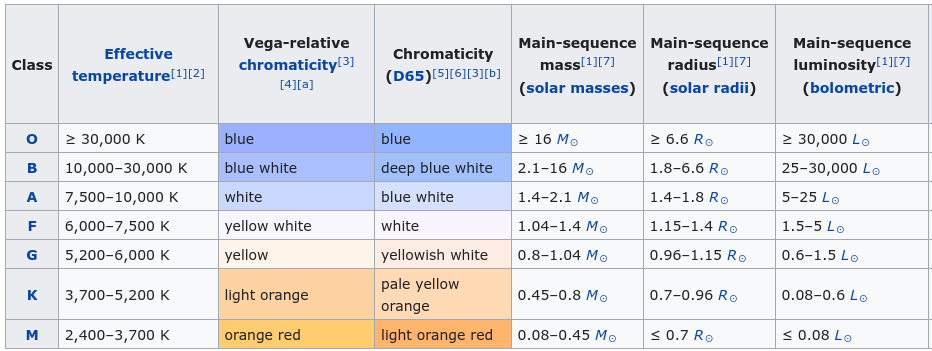
\includegraphics[scale=0.30]{latent_spectral.png}
        \caption{Harvard Spectral Classification \\ 
        Source: \url{https://en.wikipedia.org/wiki/Stellar_classification}}
        \label{fig:latent_spectral_relation}
    \end{figure}
\end{frame}


\begin{frame}{Star Classification: Is spectral type a problem?}
    Figure \ref{fig:latent_spectral_relation} shows spectral type's dependence on temperature, radius, and luminosity.
    So we need to ask ourselves if spectral type will be a problem in our model.
    
    Kind of. Consider the Hertzsprung-Russell (HR) diagram:
    \begin{figure}
        \centering
        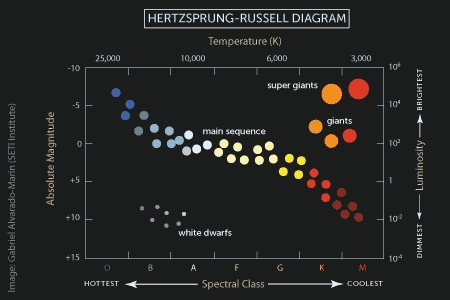
\includegraphics[width=0.72\textwidth]{hr.jpg}
        \caption{Hertzsprung-Russell Diagram}
        \label{fig:hr_diagram}
    \end{figure}
\end{frame}

\begin{frame}[fragile]{Implementation}
\begin{verbatim}
from sklearn.model_selection import train_test_split
from sklearn.discriminant_analysis import LinearDiscriminantAnalysis \
    as LDA
from sklearn.metrics import accuracy_score

X, y = data.drop(columns=['Spectral class','Star type']), 
                    data['Star type']

# Split data into 70% train, 30% test
X_train, X_test, y_train, y_test = train_test_split(X, y, 
    train_size=0.7, random_state=0)

model = LDA()
model.fit(X_train, y_train)
predicted = model.predict(X_test)

print("Model accuracy:", accuracy_score(y_test, predicted))

    >>> Model accuracy: 0.9861111111111112
\end{verbatim}
\end{frame}

\begin{frame}[fragile]{More Robust Accuracy Analysis}
    \begin{verbatim}
def LDA_error(X, y, train_size, random_state):
  # Define train and test sets
  X_train, X_test, y_train, y_test = train_test_split(X, y, 
           train_size=train_size, random_state=random_state)
  model = LDA().fit(X_train, y_train)
  return accuracy_score(y_test, model.predict(X_test))

n_iter = 50
errors = [LDA_error(X, y, train_size=0.7, random_state=seed) 
          for seed in range(n_iter)]

print(f"Model accuracy over {n_iter} splits")
print("Mean:   ", np.mean(errors))
print("Std dev:", np.std(errors))

    >>> Model accuracy over 50 splits
    >>> Mean:    0.9886111111111111
    >>> Std dev: 0.011348165675453048
\end{verbatim}
\end{frame}

\begin{frame}{Just because we were curious...}
    What happens if we project the data to 2D? Here's what we found:
    \begin{figure}
        \centering
        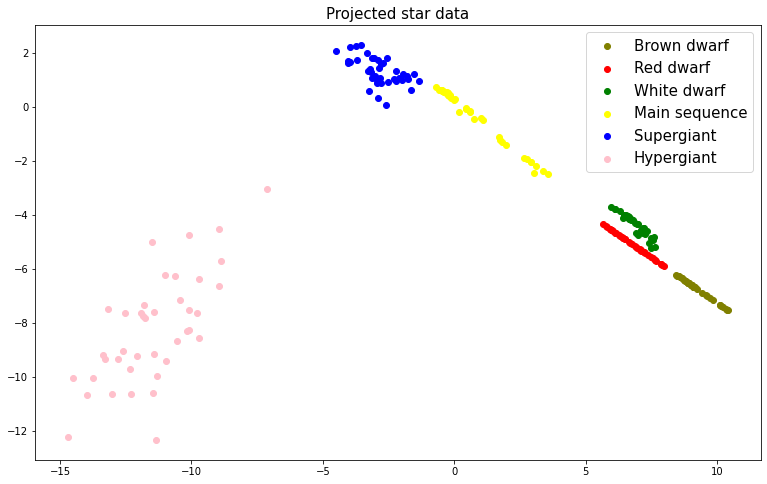
\includegraphics[scale=0.35]{hr_lda.png}
        \caption{LDA Projection of star data. It looks a bit like we've reconstructed a HR diagram!}
        \label{fig:lda_star_red}
    \end{figure}
\end{frame}

\section{LDA for Dimensionality Reduction}
\frame{\sectionpage}
\subsection{Comparison with PCA}
\frame{\subsectionpage}
\begin{frame}{Why Supervise Dimensionality Reduction?}
    \textbf{Given our knowledge of other dimensionality reduction algorithms like PCA, how is LDA different and what benefits does it provide?}
    
    Rather than explain the theoretical differences between the two algorithms, we will instead demonstrate how they perform on a toy dataset. We will be using the familiar Red Wine Quality dataset, which is built in to scikit-learn. 
    
    \footnotesize
    [Note: The difference between the built-in dataset and the one we used in Project 1 is that the target variable, wine quality, is split into three classes (low, medium, and high) based on their scores.]
    \normalsize
    
    The target variable, wine quality, depends on 13 attributes, including alcohol content, color and hue, and the concentrations of various chemical compounds. We will reduce the 13-dimensional feature vectors down to 2 dimensions and plot the results.
\end{frame}

\begin{frame}[fragile]{The Code}
    \begin{Verbatim}[fontsize=\small]
from sklearn.datasets import load_wine
from sklearn.discriminant_analysis import LinearDiscriminantAnalysis \
    as LDA
from sklearn.decomposition import PCA

# Load and separate data
wine = load_wine()
X, y = wine.data, wine.target

models = [LDA(n_components=2), PCA(n_components=2)]
proj = [m.fit_transform(X, y) for m in models]

# Plot the projected data
fig, ax = plt.subplots(1, 2, figsize=(19, 10))
model_names = ['LDA', 'PCA']
colors = ['red', 'blue', 'darkorange']
for i in range(2):
    for label in range(3):
        ax[i].scatter(proj[i][y==label][:,0], proj[i][y==label][:,1], 
                      color=colors[label])
    ax[i].set_title(model_names[i] + " Projection", fontsize=18)
fig.show()
    \end{Verbatim}
\end{frame}
\begin{frame}{The Results}
    \begin{figure}
        \centering
        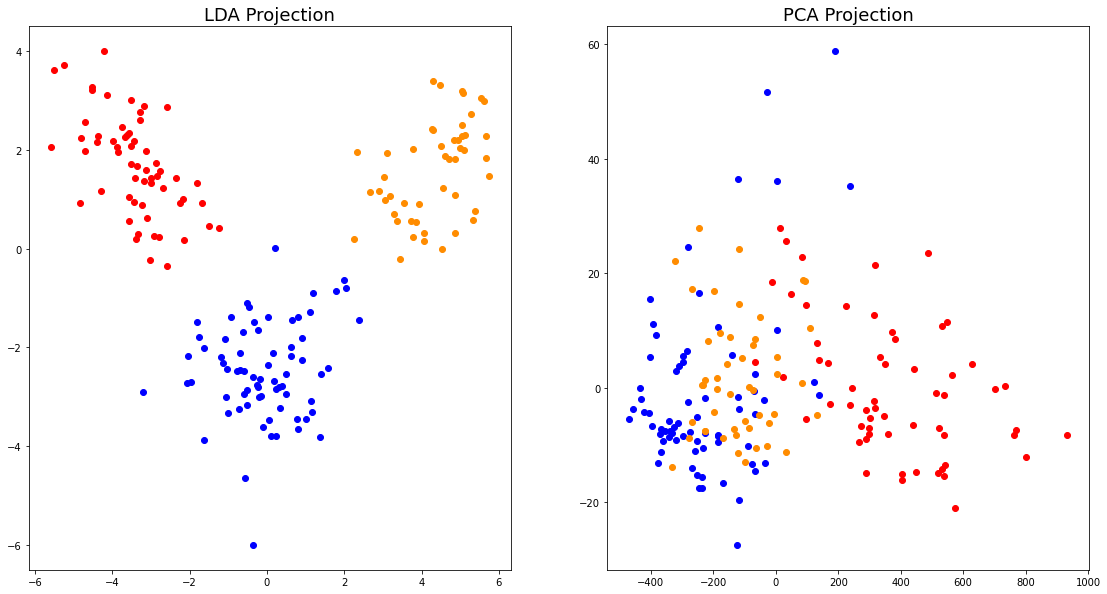
\includegraphics[height=0.55\paperheight, width=\textwidth]{pca_lda.png}
        \caption{LDA and PCA projection of the Red Wine dataset}
        \label{fig:LDAvsPCA}
    \end{figure}
    You can see the presence of the class labels accomplished something entirely different to PCA. 
\end{frame}
\begin{frame}{Why so different?}
    While PCA finds a projection subspace that aims to preserve what sets each data point apart from all the other data points, LDA does the exact opposite.
    With LDA, we \textit{want} the data points to be grouped together according to their class labels, so variance is necessarily destroyed in the projection process.
    The following figure illustrates the difference in chosen subspaces:
    \begin{figure}
        \centering
        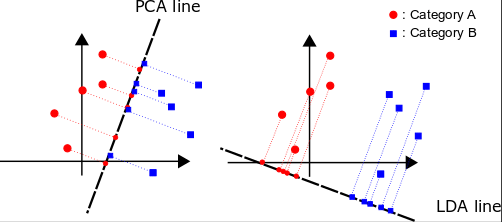
\includegraphics[width=\textwidth]{pca_lda_projectionss.png}
        \footnotesize \caption{The projection subspaces in this example are nearly orthogonal\\
        \tiny Credit: Th\'eriault et al.}
        \label{fig:my_label}
    \end{figure}
\end{frame}

\subsection{Pushing the Limits of LDA: Chest X-Rays}

\frame{\subsectionpage}

\begin{frame}{Problem}
    \setstretch{1.618}
    \begin{itemize}
        \item We use LDA-based dimensionality reduction to diagnose patients with pneumonia based on chest X-ray images. Our training set of 5000 images labels X-rays with \textbf{normal}, \textbf{bacterial pneumonia}, and \textbf{viral pneumonia}.
        \item Two-Stage Training Model:
        \begin{enumerate}
            \item Retain initial classifications and run LDA to project data to two dimensions.
            \item Group bacterial and viral pneumonia under the same class, and train three different binary classifiers (logistic regression, LDA, and SVM) on the transformed training set. 
        \end{enumerate}
    \end{itemize}
\end{frame}

\begin{frame}{Viewing the Data}
    \begin{figure}[h]%
    \centering
    \subfloat{{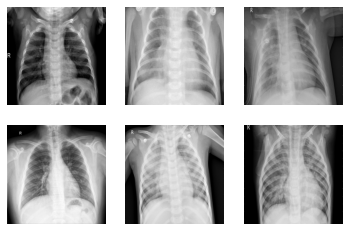
\includegraphics[width=0.4\paperwidth]{X-rays.png} }}%
    \qquad
    \subfloat{{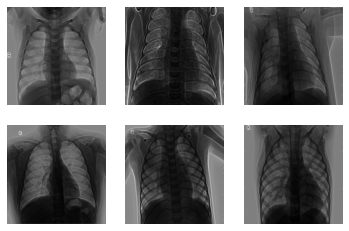
\includegraphics[width=0.4\paperwidth]{X-ray negs.png} }}%
    \qquad
    \caption{Originals and negatives of X-ray samples}
    \end{figure}
\end{frame} 

\begin{frame}{Preprocessing}
    \begin{figure}[h]%
    \centering
    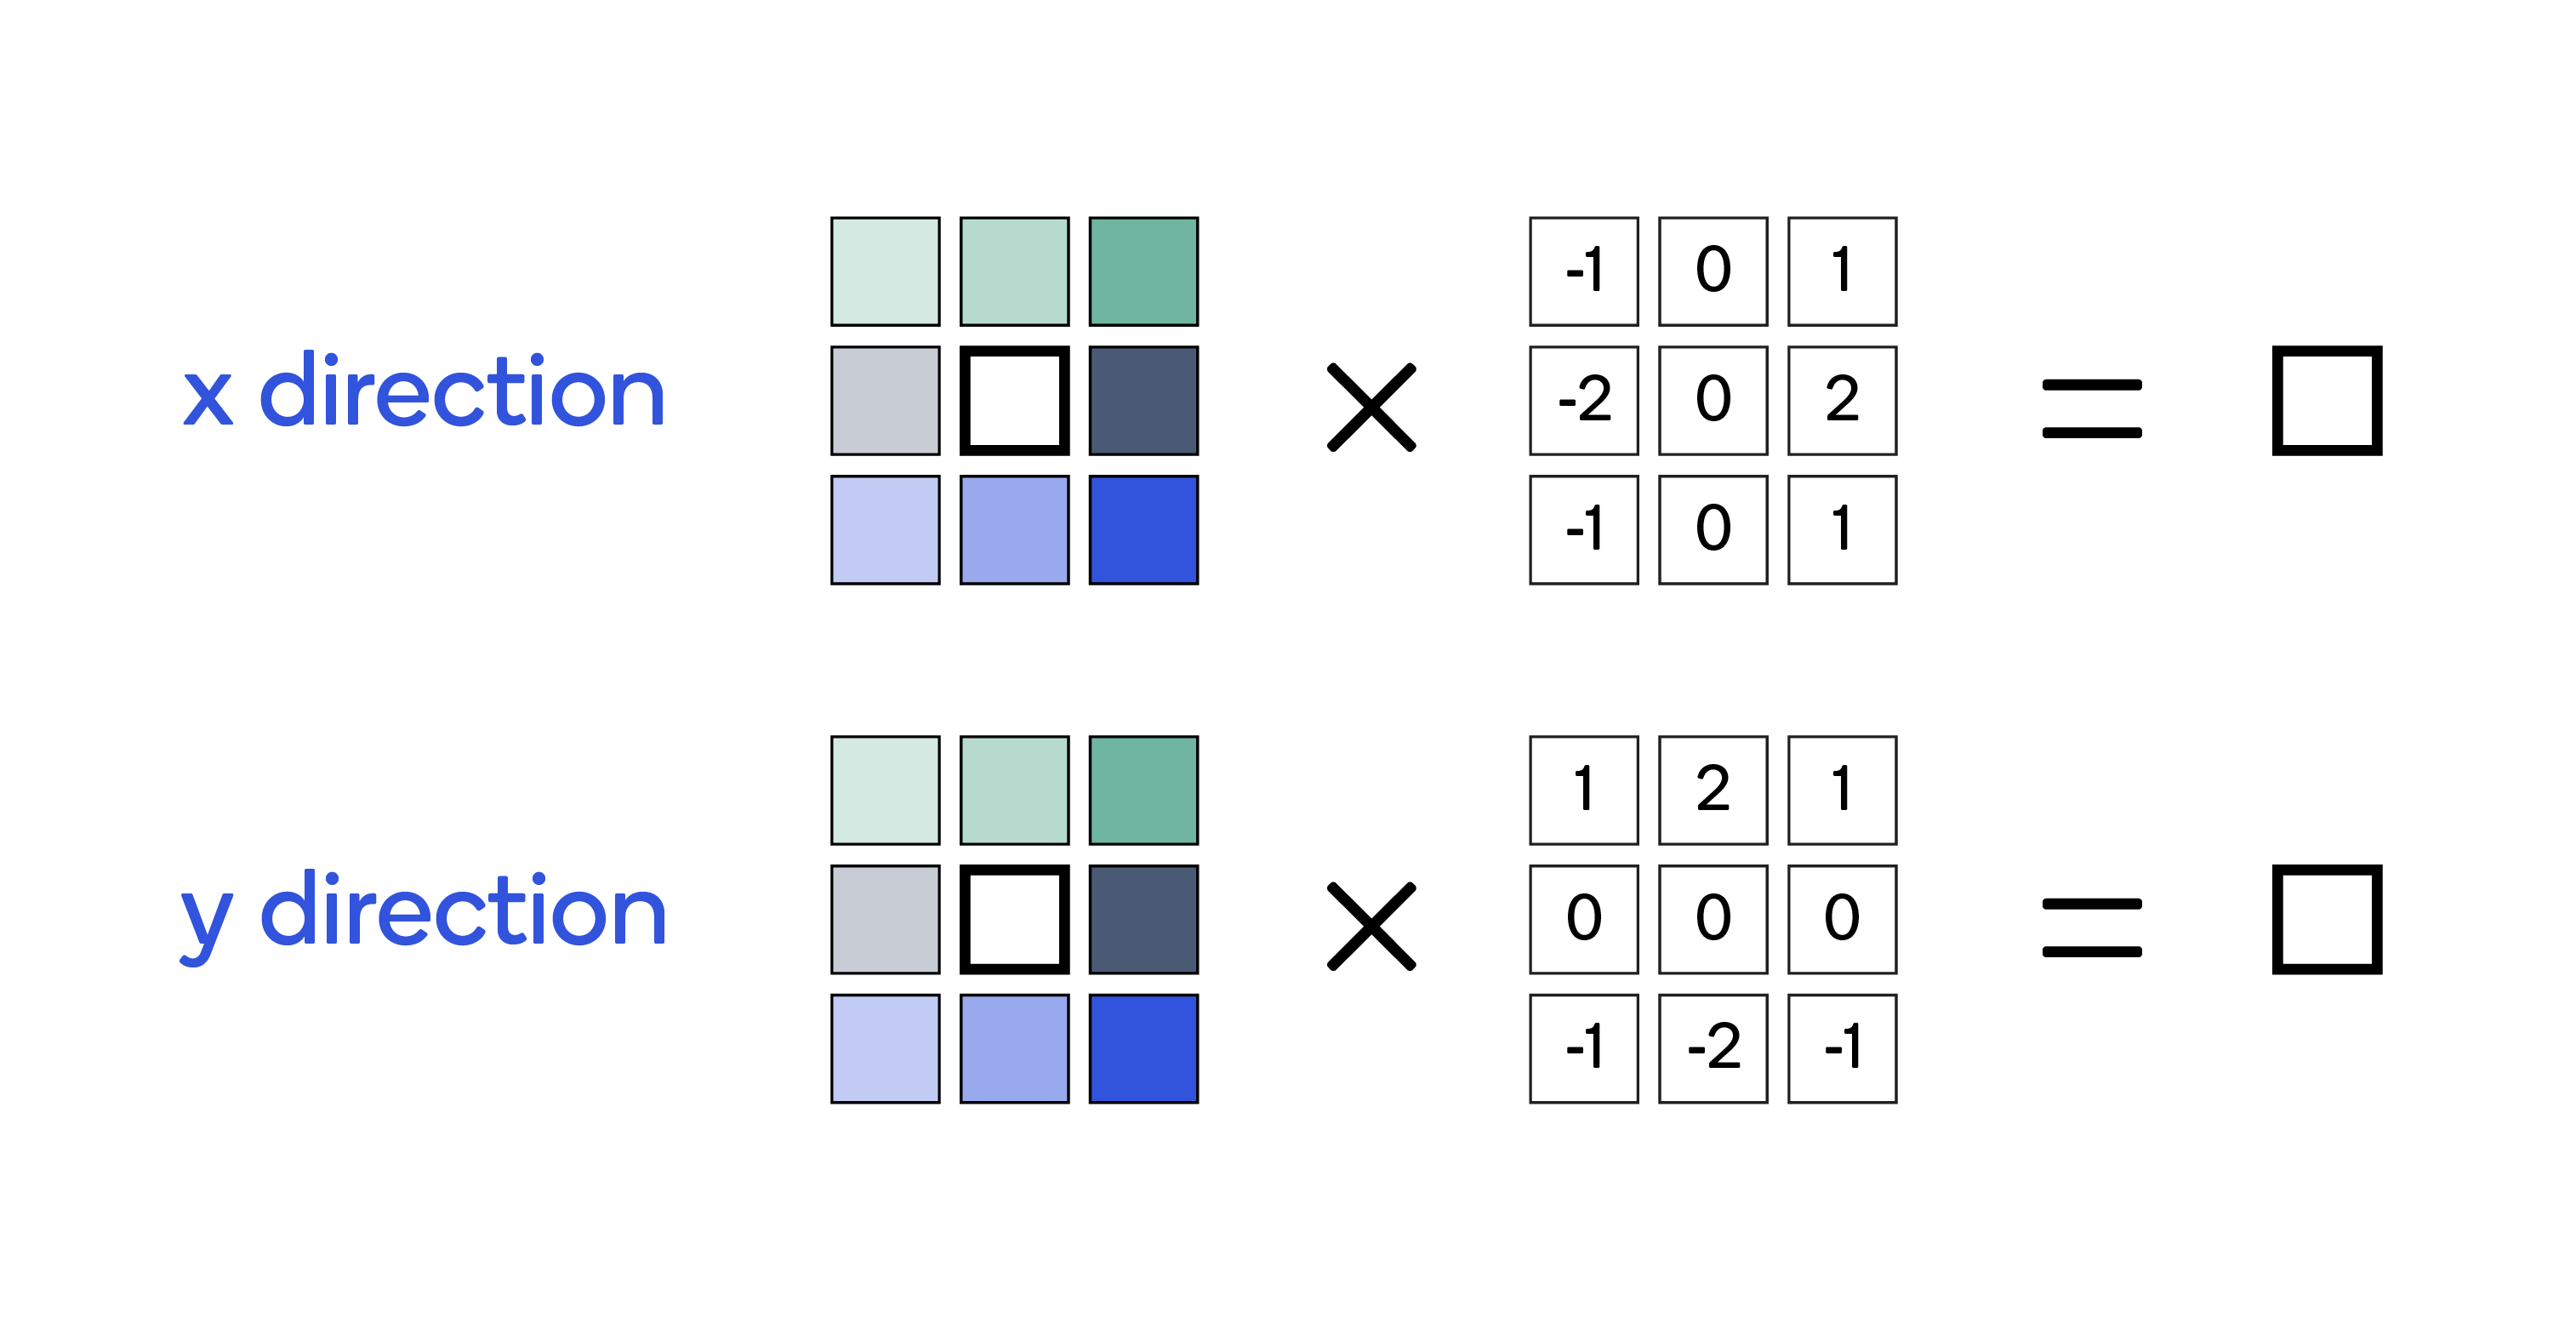
\includegraphics[width=0.6\paperwidth]{sobel_1.png}
    \caption{Applying the Sobel Filter \\ Source: \url{https://developer.qualcomm.com/sites/default/files/attachments/}}
    \end{figure}
\end{frame}
\begin{frame}{Projection Results}
    \begin{figure}[h]%
    \centering
    \subfloat{{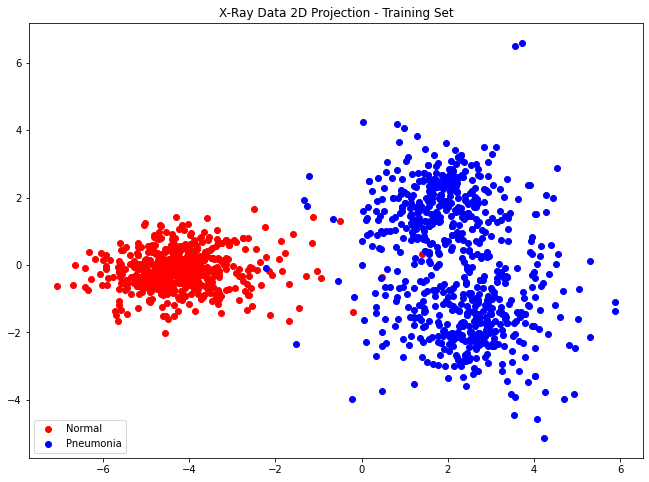
\includegraphics[width=0.4\paperwidth]{X-ray proj.png} }}%
    \qquad
    \subfloat{{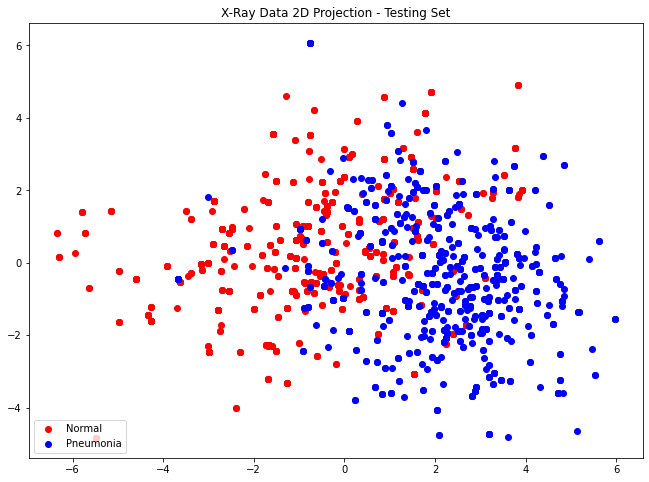
\includegraphics[width=0.4\paperwidth]{X-rayprojtest.png} }}%
    \qquad
    \end{figure}
For all three second-stage binary classifiers, the accuracy of our two-stage model was approximately 95\% for the training set and 70\% for the testing set. By preprocessing the images with a Sobel filter, our test accuracy improved to 75\%.
\end{frame}
\begin{frame}{Thanks for listening!}
    \begin{center}
        \textbf{Feel free to ask questions now or on Campuswire!}
        
        Our full code and presentation material is available on a Github repository here: \url{https://github.com/warewaware/LDAFinalProj}
    \end{center}
\end{frame}
\end{document}
